\documentclass[10pt]{sigplanconf}

\usepackage{amssymb}
\usepackage{amsmath}
\usepackage{amsfonts}
\usepackage{graphicx}
\usepackage{url}
\usepackage{xspace}
\usepackage{listings}
\usepackage[noline]{algorithm2e}
\usepackage{comment}
\usepackage{color}
\usepackage{times}
\usepackage{multirow}
\usepackage{balance}
\usepackage{adjustbox}
\usepackage{alltt}
\usepackage{textcomp}
\usepackage[usenames]{xcolor}

\setcounter{tocdepth}{3}


% configures style of source code listings
\lstset{
	basicstyle=\small\sffamily
	%basicstyle=\scriptsize\ttfamily
	%numbers=left
}

\lstdefinelanguage{java}{
	morekeywords={abstract,continue,for,new,switch,assert,default,goto,package,synchronized,boolean,stream,event,filter,when,do,if,private,this,break,double,implements,protected,throw,byte,else,import,public,throws,case,enum,instanceof,return,transient,catch,extends,int,short,try,char,final,interface,static,void,class,finally,long,strictfp,volatile,const,float,native,super,while},
	sensitive=false,
	morestring=[b]",
	morestring=[b]',
	morecomment=[l]{//},
	morecomment=[s]{/*}{*/)},
	escapeinside=??,
	moredelim=[is][\textit]{__}{__},
	moredelim=[is][\textbf]{_*}{*_}
}
\lstnewenvironment{displayjava}
	{\lstset{language=java,basicstyle=\small\sffamily,tabsize=2,columns=fullflexible,captionpos=b,xleftmargin=1em,xrightmargin=1em}}{}
\lstnewenvironment{java}
	{\lstset{language=java,basicstyle=\small\sffamily,tabsize=2,columns=fullflexible,captionpos=b}}{}


\newcommand{\code}[1]{{\sf \small #1}\xspace}

\newcommand{\mi}[1]{\mathit{#1}}
\newcommand{\mr}[1]{\mathrm{#1}}
\newcommand{\mt}[1]{\mathtt{#1}}

\newcommand{\todo}[1]{{\bfseries #1}}

% for writing comments
\newcommand{\PP}[1]{\textcolor{blue}{\bfseries PP: #1}} % Pavel Parizek
\newcommand{\PV}[1]{\textcolor{red}{\bfseries PV: #1}} % Premek Vysoky
\newcommand{\JB}[1]{\textcolor{orange}{\bfseries JB: #1}} % JetBrains

% colors for the ANTLR environment
\definecolor{antlrbgcolor}{rgb}{.962, .962, .962}
\definecolor{antlrparserrulecolor}{RGB}{11,83,148}
\definecolor{antlrlexerrulecolor}{RGB}{191,144,0}
\definecolor{antlrliteralcolor}{RGB}{133,32,12}
\definecolor{antlrregexcolor}{RGB}{56,118,29}

% colors for the MPS environment
\definecolor{mpsbgcolor}{rgb}{.962, .962, .962}
\definecolor{mpsconceptcolor}{RGB}{42, 140, 0}
\definecolor{mpsinterfacecolor}{RGB}{170,0,229}

% coloring commands
\newcommand{\antlrap}{\textquotesingle}
\newcommand{\antlrparserrule}[1]{\textcolor{antlrparserrulecolor}{#1}}
\newcommand{\antlrlexerrule}[1]{\textcolor{antlrlexerrulecolor}{#1}}
\newcommand{\antlrliteralnoap}[1]{\textcolor{antlrliteralcolor}{#1}}
\newcommand{\antlrliteral}[1]{\antlrap\antlrliteralnoap{#1}\antlrap}
\newcommand{\antlrregex}[1]{\textcolor{antlrregexcolor}{#1}}
% TODO mozna zmenit "mpsconcept" na "mpslangelem"
\newcommand{\mpsconcept}[1]{\textcolor{mpsconceptcolor}{#1}}
\newcommand{\mpsinterface}[1]{\textcolor{mpsinterfacecolor}{#1}}

% TODO zmenit barvu pozadi na bilou
% environment for the ANTLR code (grammars)
\newenvironment{antlr}
{
	\vspace{3mm}
	\par
	\noindent
	\adjustbox{margin=3mm,bgcolor=antlrbgcolor,frame,minipage=394pt,inner=\linewidth}
	\bgroup
	\alltt
}
{
	\endalltt
	\egroup
	\\
	\vspace{2mm}
}

% environment for the MPS code
\newenvironment{mps}
{
	\vspace{3mm}
	\par
	\noindent
	\adjustbox{margin=3mm,bgcolor=mpsbgcolor,frame,minipage=394pt,inner=\linewidth}
	\bgroup
	\alltt
}
{
	\endalltt
	\egroup
	\\
	\vspace{2mm}
}



\begin{document}


% TODO
%\conferenceinfo{OOPSLA'12,} {October 19--26, 2012, Tuscon, Arizona, USA.}
%\CopyrightYear{2012}
%\copyrightdata{978-1-4503-1561-6/12/10}


% TODO
\title{\todo{INGRID: Creating Languages in MPS by Importing ANTLR Grammars}}
% alternative: "INGRID: Importing Grammars Into MPS"


\authorinfo{P\v{r}emysl Vysok\'y \and Pavel Par\'izek}
	{Charles University, Faculty of Mathematics and Physics, Prague, Czech Republic}
	{premek.vysoky@gmail.com, parizek@d3s.mff.cuni.cz}

% TODO pridat nekoho dalsiho z JetBrains
% TODO upravit affiliation pro JetBrains -> doplnit "s.r.o" nebo radsi "Inc."
% TODO muzeme taky napsat jejich emaily pokud budou lidi z JetBrains souhlasit
\authorinfo{V\'aclav Pech}
	{JetBrains}


\maketitle

\begin{abstract}
% TODO
\todo{write later}

\todo{Copy from master thesis.}
JetBrains MPS is a language workbench focusing on domain-specific languages.
Unlike many other language workbenches and IDEs, it uses a projectional editor for code.
The developer directly manipulates the program in its tree form (AST) and not by editing a text source code.
This brings many advantages, but on the other hand requires time-consuming and complicated MPS language definition.
The thesis elaborates on the possibility of automating the process of creating MPS language definition from its grammar description.
It introduces the MPS editor, evaluates approaches of related projects and describes author's efforts to implement an MPS plugin that allows this import.
The chosen approach and the selection of tools used for implementation are justified in the thesis.
We point out important problems that any similar project might deal with and we introduce some possible solutions.
Furthermore, the thesis contains examples of imported languages, showing the potency of the chosen approach.
The thesis also aims to lay groundwork for future extensions and suggest possible improvements.
\end{abstract}

% TODO possible keywords: JetBrains MPS, programming language, grammar, projectional editor



\section{Introduction}

\JB{Odstavec mirne upraven} The prevailing approach to define valid syntaxes for programming languages is through grammars written typically in notations based on (or similar to) EBNF [reference]. Many popular tools exist for automated generation of parsers from the grammar definitions, such as ANTLR and Bison/Flex. The source code of programs in such languages is written in a text editors, usually embedded into an IDE.

\JB{Odstavec mirne upraven} Projectional (or structural) editing offers an alternative approach. While the idea emerged as early as in 1970s, it failed to get adopted widely, mostly due to inconvenient and unnatural way of manipulating code.  A recent revival of projectional editing has been observed in the area of language workbenches - IDE-like tools that enable the developers to manipulate the actual language definition. The Meta-programming System (MPS) [reference] by JetBrains is an open-source language workbench that focuses of Domain Specific Languages and leverages the concept of projectional editor. MPS allows developers to design custom languages and then use use them to write code and compile it into executables. MPS provides the whole IDE infrastructure for such languages.

\JB{Odstavec mirne upraven} The key idea behind projectional editors is that a developer directly manipulates the AST representation of the source code instead of plain text. To avoid the fate of the early projectional editors MPS has put extra effort into making text manipulation feel like editing real text. MPS models, although being persisted as XML or binary files, can be versioned using the industry standard source-control systems (Git, Subversion). On-line model browsers have been incorporated into some of the popular public source code repositories (BitBucket) [reference] .

\JB{Odstavec mirne upraven} The absence of parsers brings about numerous benefits, which are in particular useful for DSLs, which are frequently used by domain experts, who may not be professional programmers.
\begin{itemize}
	\item Since a projectional editors controls the interaction between the user and the code, the developers practically cannot enter syntactically invalid code.
	\item Languages can be defined in a modular way and multiple languages can be easily combined together or extend one another, while parsers seriously limit language modularity for traditional parsed languages.
	\item The languages may offer contextual or non-parseable notations, such as tables, diagrams or positional syntax.
	\item Since the projection is detached from the physical representation of code (AST), authors can define multiple notations and allow the developers to switch between different representations of the code.
\end{itemize}
A motivating illustration of the abilities of MPS is the mbeddr project [citation], which extends C with numerous domain-specific constructs and data types.
We provide more details about MPS in Section 2.1.

\JB{Navrhuji smazat nasledujici odstavec}
\todo{From thesis.
	One of these tools is the JetBrains MPS~\cite{ref:MPS}, which approaches languages from a~different point of view.
	MPS doesn't use the textual representation of code as usual, but rather works with the actual abstract syntax tree that holds the code's structure.
	This has some positive implications as it gives us a~very powerful tool rich on features but also introduces some new problems we haven't encountered before.
	One of them being the need for a~special definition of languages created inside MPS so that the IDE can understand them and work with them.
	MPS also becomes a~very powerful tool once the language has already been created and you start using it inside MPS.
	There is a~huge variety of new languages constructed for MPS that usually solve domain specific problems.
}

\todo{Pouzivat jen terminy "AST nodes" a "language elements" (to spis). Nepouzivat pojem "concepts" abychom ctenare nematli.}

\JB{Odstavec upraven} Projectional editing introduces some new problems we haven't encountered before. One of them is the need for a~special definition of languages created inside MPS so that the IDE can understand them and work with them. In order to use a language inside MPS, it has to be defined through the MPS infrastructure. In particular, one has to create the abstract syntax called Structure (the types of allowed AST nodes), concrete syntax called Editor (projection of the AST on the screen and its interactions with the user), and text generation (to enable creation of plain text files used as input for compilers). We provide more details in Section X (Background about MPS).

\JB{Odstavec pridan pro vysvetleni motivace prace} MPS is typically used for syntactically rich DSLs, which are likely to benefit most from overcoming the limitations of parser-based languages. These DSLs are then transformed on the AST level by a series of model-to-model transformations to an AST model representing the desired semantics in a General-purpose language (GPL), such as C or Java. This model is then converted to a textual representation of that language and compiled by the standard means of the target platform. This implies that the target GPL must also be defined by the MPS means, to allow the DSLs to have their models transformed into a model in the GPL.

\JB{Odstavec doplnen} However, it requires substantial effort to create a definition of a GPL in MPS. Therefore, very few mainstream GPLs are now fully supported by MPS. Only Java and C have been implemented to date, which limits the DSLs authors to only target these supported target GPLs. We believe that an automated process of importing grammars of GPLs into MPS would encourage more GPLs to be migrated to MPS and thus giving the DSL authors more options.

\todo{From thesis.
	However, building these languages is a~complicated and time-consuming process and a~lot of effort must be put into them before they are ready for use.

	These examples show that recreating a~full language inside MPS is not an easy task and a~lot of time must be spent on implementing all aspects of the language.
	A big part of this effort is, however, quite straightforward and can be possibly automated, as we show in this paper. Automation speeds up the process of adoption of new languages to a great degree.
}

\JB{Odstavec upraven} Since a big part of the language definition process in MPS is quite straightforward and can possibly be automated, we will look into the possibility of automatic import of already existing general purpose languages into MPS using a grammar description of their syntax.

We present INGRID --- a method and a tool for semi-automated construction of MPS definition of programming languages based on their ANTLR grammars.
We also discuss challenges that we encountered during this process and our solution to them. Most of these challenges are general, i.e. not MPS specific, as they apply to the relation between grammars defined in EBNF-like style (rules and tokens, everything defined in plain text) and structured (object-oriented) approach used in MPS (and other language workbenches).

\todo{Hodne zduraznit automation, tedy ze chceme maximalizovat automatizaci.}
The main goal of our/the INGRID approach is to automatize the construction of MPS languages from ANTLR grammars as much as possible.

\todo{From thesis.
	Automatic import of already existing languages into MPS from the grammar description of their syntax.
}
\todo{Mozna prodat INGRID jako automatickou konverzi gramatik do podoby MPS languages, tedy jako nastroj ktery umoznuje portaci jazyku do prostredi MPS a jejich nasledne pouziti v MPS (treba kombinace s dalsimi jazyky).}

Our primary motivation is to enable better support for mainstream and/or general purpose programming languages (XML, C, C++, JavaScript, Python) in MPS, especially to enable writing programs in these languages using the projectional editor and to combine them with domain-specific languages natively created in MPS.
\todo{Zduraznit take pouziti importovanych jazyku pro cile generovani z DSL --- to plati zejmena u mainstream general-purpose languages jako treba JavaScript.}

\todo{Briefly mention the biggest challenges.}
The are related to the way grammar encoding/description of languages are usually written.
They do not hold any information about the code layout, and contain many rules that do not directly correspond to AST nodes (programming language constructs).
We discuss them in more detail later (Section X).

\todo{From thesis.
	INGRID allows developers to leverage all the features that MPS has to offer together with general purpose languages such as C++, JavaScript or Python.
	The biggest benefit is the possibility to code in these mainstream general purpose languages using the projectional editor.
}

However, we do not target just the very complex general purpose languages such as JavaScript.
INGRID can be used also for simple languages.
We believe that, for simple languages, it is less time consuming to create the grammar by hand (e.g., using the ANLTR notation and toolset) and then create the language definition in MPS by using the INGRID tool, than to create it manually using the MPS GUI --- this is another benefit of INGRID.

Structure of the paper.
In the beginning, we will describe the MPS editor and related/similar projects.
Then, we describe our approach to creating language definition in MPS from their grammars, and discuss the major challenges together with our solution.
We will also show some example languages imported with INGRID and discuss our experience.


\section{Background and Related Work}

We will briefly introduce fundamental basics of the MPS environment.
We will analyze existing related projects that are trying to accomplish similar goals, and then we will weigh advantages and disadvantages of these approaches.

\subsection{JetBrains MPS}

\JB{Odstavec upraven} JetBrains MPS is a complete language workbench - a development environment that allows developers to define their own languages and then use them to develop code. The code can then be transformed into a target language, typically a GPL, such as Java or C.

\JB{Navrhuji odstranit} We need to provide a good understanding of how the MPS~\cite{ref:MPS} environment works.
Focus on basic/fundamental and relevant features. In this section, we will explain fundamental basics of MPS as it is crucial in the understanding of our contribution and associated challenges.

\JB{odstavec upraven} MPS differs from typical IDEs in one important aspect - the projectional editor. The developer does not work with the textual representation of the source code directly, but rather with its AST (abstract syntax tree) that is the model of the code. When users are creating programs using the MPS projectional editor, they are basically assembling the tree (AST) out of predefined building blocks of the imported languages. The definition of the language dictates, which where in the AST can certain elements be placed or how they can be nested inside other elements. In traditional IDEs it is the parser that constructs an AST using the language's elements.

\JB{Odstavec upraven} The building blocks of MPS models are called nodes. Code of any program in MPS is built from nodes and these nodes represent instances of elements defined in one of the languages that the program declares to be using. These language elements are called concepts. In brief, nodes in code are instances of concepts defined in the language.

\JB{Vyhody/nevyhody diskutujeme v kapitole 1. Navrhuji nasledujici odstavec zrusit nebo text z kapitoly 1. presunout sem}
Keeping the model of the code in the AST form has several advantages.
One of them is that MPS then only allows composing the program strictly following the syntax of the language, which results in an inability to actually write syntactically invalid code.
The code is generated out of the always-valid AST beyond user's reach.

\JB{Odstavec upraven} One of key advantages of projectional editor stems from separation of abstract and concrete syntax. While the AST provides an exhaustive representation of the code, the way it is displayed on the screen and the way the user interacts with it are unconstrained. The editor can take any visual form and shape. The language author can define multiple visualizations and let the developer to choose one that fits best the task at hands - editing, debugging, reviewing, resolving merge conflicts, etc.

For a better understanding, we will give a~small example. Let's assume we have a language with typical if/else structure similar to the one in Java:

\begin{center}
	\begin{minipage}{.38\textwidth}
		\begin{alltt}
			if (\textit{condition})
			    \textit{then statement block}
			else
			    \textit{else statement block}
		\end{alltt}
	\end{minipage}
\end{center}

Its abstract syntax tree representation will look something like shown on Figure~\ref{fig:if_ast}.

\begin{figure}[ht]
  \centering
  \includegraphics[scale=0.6]{./images/if_statement_ast.png}
  \caption{"If statement" abstract syntax tree}
  \label{fig:if_ast}
\end{figure}

The underlying child nodes have their own children and so on. The type of nodes can be restricted by the language structure definition. For example, we can restrict the condition in the if/else statement to be an expression, the statement block to be a list of statements, etc.

\JB{odstavec upraven} Alternative visual representations are possible and they are not bound to be just the textual representation at all. For example, blocks for both of the branches can be aligned next to each other and displayed with differend background color, like shown in Figure~\ref{fig:if_editor}.

\begin{figure}[ht]
	\centering
	\hspace{-4mm}
	\includegraphics[scale=0.75]{./images/if_statement_editor.png}
	\caption{"If statement" projectional editor example}
	\label{fig:if_editor}
\end{figure}

\JB{Odstavec mirne upraven}The definition of a language element (the concept) consists of several aspects and each aspect codifies a different part of the nodes' behavior. The essential aspects are the following: structure (abstract syntax), editor (concrete syntax - how the code is projected and edited) and textgen (how to transform the AST into textual source code). If, instead of generating text directly, the language is supposed to be generated into another language that is available in MPS, the generator aspect must be used to specify the model-transformation rules. The structure, editor and textgen aspects are most relevant for the contribution of this paper, so we describe them here (and neglect/ignore the other aspects such as type system and data-flow).

\todo{Highlight the object-oriented hierarchical nature of language definitions in MPS. The environment restricts and guides the developer so that he makes less mistakes.}

Some concepts and design patterns known from object oriented programming can be used in language definition for MPS --- inheritance between concepts, interfaces, delegation and so on. Most importantly, nodes can have child nodes and that is how the AST itself is created.

\JB{Zmineno vyse, navrhuji odstranit} \todo{Zduraznit ze AST node (object) ma nekolik aspectu: structure, editor, textgen. Definice MPS language je organizovana takto --- pres AST nodes, ktere maji nekolik aspectu (ruzne pohledy).}

\paragraph{Structure.}
\JB{Odstavec mirne upraven} The fundamental aspect of any MPS language is structure. It must be created first for each type of the intended AST node. Structure specifies core attributes such as name of the concept, inheritance relationships, possible child concepts (their types and cardinalities), the implemented interfaces, references to other nodes, other properties (fields of any type that can hold values), etc.
In Figure~\ref{fig:if_statement_structure}, you can see the structure aspect definition for the if statement.

\begin{figure}[ht]
	\centering
	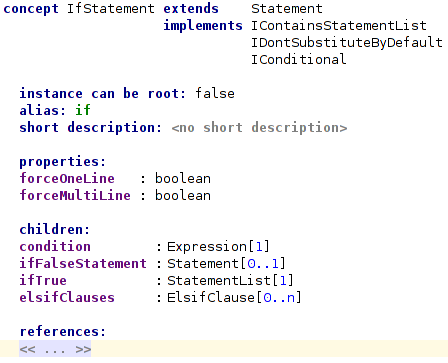
\includegraphics[scale=0.55]{./images/if_statement_structure.png}
	\caption{"If statement" structure aspect definition}
	\label{fig:if_statement_structure}
\end{figure}

\paragraph{Editor.}
\JB{Odstavec mirne upraven}The editor aspect is where the user defines what the projectional editor representation of a code fragment (an AST node) looks like on the screen and how the user interacts with the code. JetBrains have developed a cellular system that allows placing node's (concept's) properties and children into different cells. The author usually incorporates all concept's children, references, and properties inside the representation so that the future users of the language can insert the values that the node expects. Additionally, all visual cells of the editor can be styled using a~language similar to CSS.

\begin{figure}[ht]
	\centering
	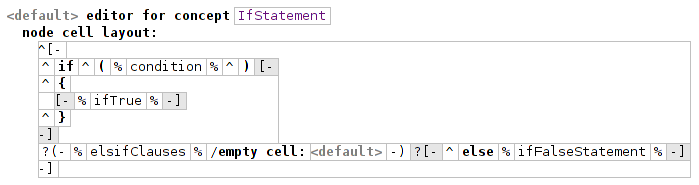
\includegraphics[scale=0.5]{./images/if_statement_editor_definition.png}
	\caption{"If statement" editor aspect definition}
	\label{fig:if_editor_definition}
\end{figure}

\JB{Nasledujici odstavec navrhuji odstranit}
\todo{From thesis.

The editor is a module dedicated/responsible for the definition of appearance of an AST node (concept).
JetBrains have developed a cellular system that allows placing node's (concept's) properties and children into different cells.
These cells then can be styled to user's liking.
There are many different types of cells, each behaving a little bit different towards its contents.
For example, MPS supports various horizontal and vertical lists, etc.
Extra cells can be added on top --- cells which just specify layout adjustments such as indentation and text color.
In Figure~\ref{fig:if_editor_definition}, you can see what a real editor definition might look like for the if statement of the Java language (as defined in MPS).
}

\paragraph{BaseLanguage}
\todo{Introduce the base language here.}
\JB{Odstavec prepsan}
In order to implement MPS itself and also to support the basic set of language-definition DSLs, BaseLanguage was developed in the early days of MPS. BaseLanguage is a clone of Java implemented using the MPS constructs. Although BaseLanguage is syntactically almost identical to Java, it is edited in a projectional editor, just like all languages in MPS. The DSLs that language authors use in order to define languages are generated into BaseLanguage. Similarly, all customer DSLs that are meant to be generated into Java choose BaseLanguage as their generation target and the conversion to textual Java will be handled by BaseLanguage without any further effort, since BaseLanguage has a TextGen aspect defined, which translates BaseLanguage code into textual Java sources.

\paragraph{TextGen.}
\JB{Odstavec upraven} The TextGen aspect defines how a certain AST node will be translated into text. The TextGen aspect is typically only needed for the bottom-line (base) languages. DSLs, on the other hand, need to define rules for model-to-model conversion (a generator), since these are rarely converted to text directly. After TextGen has generated textual sources from an AST, a compiler for the particular GPL gets invoke in order to compile the generate sources into binary code.
The TextGen definition follows a very straightforward pattern - each node outputs its textual representation into a textual buffer, calling TextGen of its children nodes at the right moments. MPS then calls this method for the root AST nodes of the given program.
TextGen aspect has to be defined (especially its more complex functionality) using the BaseLanguage.
Again, we included an example of the if statement (Figure~\ref{fig:if_statement_textgen}).

\begin{figure}[ht]
	\centering
	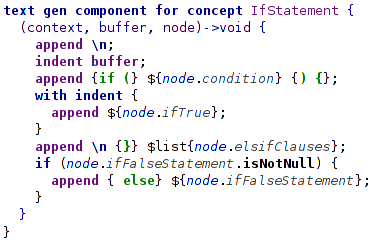
\includegraphics[scale=0.6]{./images/if_statement_textgen.png}
	\caption{"If statement" TextGen aspect definition}
	\label{fig:if_statement_textgen}
\end{figure}

\JB{Navrhuji odebrat}
\todo{From thesis.

After the program's AST is created using the projectional editor, there can be rules defined on how to generate code in plain text out of that tree.
This module is called "text gen".
These defined generators can target any language and platform.

\paragraph{Other aspects.}
MPS supports also other aspects, such as type checking, model transformations, static and data-flow code analysis, refactorings, language migrations, etc., but these are not important for our contribution. Moreover, the information needed for their automated generation is not available/contained inside a grammar file.

}

\subsection{Similar Projects}

Currently, there exists an almost full port of the Java language called BaseLanguage~\cite{ref:BaseLanguage} extended with some MPS specific features.
It was imported manually by JetBrains and it is still undergoing changes as Java itself is evolving.

Within the mbeddr project~\cite{ref:mbeddr}, the C language is also manually tailored for MPS.

Now/here we describe three similar projects (with similar goals) that we are aware of.
We focus on (consider) these three projects: PE4MPS, ANTLR{\_}MPS, and mps-metabnf.

\paragraph{PE4MPS.}
PE4MPS~\cite{ref:PE4MPS} is a project by \todo{Doplnit autora} that is trying to solve the same problem as we do.
It solves the lack of information about code layout in grammars by creating a new grammar notation called PE Grammars~\cite{ref:PE} (the PE abbreviation comes from projectional editing).
It has tw components: PE parser and PE4MPS plugin for MPS.
Their approach is to mimic an existing grammar notation called ANTLRv4~\cite{ANTLR4} and enrich its syntax with custom (their own) constructs.
These extensions tell (guide, hint) the parser what the AST node layout should look like.
Supported extensions (already implemented) include horizontal and vertical lists, and some indentation rules --- however, even these few features make the already not-so-simple syntax of ANTLR v4 much more complex.
The parser then uses this information when generating the projectional editor for am AST node.
Author of this approach/project described the PE syntax using the ANTLRv4 notation~\cite{ANTLR4reference} and then used the ANTLR toolset to automatically generate an ANTLRv4 parser for PE grammar files.
The PE parser reads any PE file and stores the language structure found inside to a custom representation of Java objects.

The PE4MPS plugin/project/tool is built on top of the PE parser.
This plugin uses the PE parser to build the PE file representation (the aforementioned tree-like structure of Java objects) and then creates AST nodes and their aspects inside MPS.
The extended syntax brought by PE describes the layout of each element, e.g. it tells the plugin that one set of child nodes should be displayed horizontally, another set should be vertical with each child on a separate line and with some indentation, and so on.

A limitation of the PE4MPS approach is that it, from what we understand, does not implement full ANTLR syntax.
This means that every grammar might need a non-trivial adjustment before its usage.
One of our goals is to enable import of as many languages out-of-the-box as possible and adopting the full specification.

\paragraph{ANTLR{\_}MPS.}
ANTLR{\_}MPS~\cite{ANTLR2MPS} is another project that is dealing with a similar problem.
The author of this project is Fabien Campagne
The ANTLR{\_}MPS project also uses ANTLRv4 grammar notation~\cite{ANTLR4} and tries to import grammars inside MPS.
However, it does not try to generate the projectional editor at all (i.e., it does not deal with this problem), probably because it is in an early stage of development.

The way this import process of ANTLR{\_}MPS works is quite different from what we have seen in the PE4MPS project, and it is quite complex/complicated to use.
It works as follows. We give only a brief high-level overview and omit low-level technical details.
The author created a whole new ANTLRv4 MPS language, which is an MPS port of the grammar notations' syntax.
To import a language, the user utilizes this MPS ANTLR language.
The textual grammar is imported automatically into MPS taking the form of the MPS's ported grammar language (so that the textual grammar is converted into MPS nodes, that means an AST node is created for each grammar rule).
No child-parent relationships in the structure are generated by the tool --- all must be created manually by the user.
There are no editor nor TextGen aspects created neither.

\paragraph{mps-metabnf.}
\todo{Popis na zaklade emailove diskuze (Nizozemci).}


\section{Creating Language Definition in MPS}

From all the available notations in which grammars can be written, we decided to use the ANTLRv4 grammar notation~\cite{ANTLR4reference} as the input format (in which the input programming languages have to be defined) for the following reasons.
\begin{itemize}
	\item It is a very widely used grammar notation.
	\item All popular and widely used programming languages have their syntax captured (represented) using this notation --- see the repository~\cite{ref:ANTLR4grammars}.
	\item There is a whole framework/toolset for generating parsers and editing grammars built around it~\cite{ref:ANTLR4}.
	\item It supports Java (it is written in Java), which is the implementation language of MPS and also the default BaseLanguage.
	\item It uses (is based on) an EBNF (Extended Backus-Naur Form) \footnote{https://en.wikipedia.org/wiki/Extended{\_}Backus\%E2\%80\%93Naur{\_}Form} form that it useful because it meets/respects the object oriented design that is used when describing MPS aspects (definitions of MPS languages).
	\item It has its own syntax captured in its own syntax\footnote{https://github.com/antlr/grammars-v4/tree/master/antlr4} (there is an ANTLRv4 grammar for the ANTLRv4 notation). This is a very important feature as it allows us to create a parser for ANTLRv4 grammars so that we can parse grammars of other languages.
\end{itemize}

We use ANTLRv4 grammars as inputs (and work with them).
	https://github.com/antlr/antlr4/blob/master/doc/index.md
	https://github.com/antlr/grammars-v4

Unlike some of the related projects, we did not add any new features into the grammar notation.
We tried to import grammars as they are.

The generation/import process performed by INGRID consists of three phases (import of structure, usable editor, text generation).
We will talk about all phases of the generation/import process, describing encountered challenges/obstacles using an example language.

To fulfill our goal of maximal possible automation, we import/generate the full language structure and then do a lot of mundane and time-consuming work connected to creating projectional editors.

Now we describe/introduce the main steps of our approach (that INGRID tool performs): parsing the grammar, creating the structure, editor, and textgen.
We are able to create/generate the structure aspect and then very basic editor and some default/basic textgen.
In particular, we did not port the ANTLR notation as an MPS language.
In the following subsections, we provide some details about our approach to parsing the input grammar and creating the main aspects of each element (each type of AST node) of an MPS language (structure, editor, and textgen).

During our work on this project, we also discovered/encountered challenges/issues related to input grammars --- intermediate rules in the syntax hierarchy that allow humans to understand the grammar better (structure aspect/component), whitespace (editor aspect).
There is a challenge/issue that we have discovered during our work on this project (in the process of our own implementation), and that is related to construction of the structure aspect.
Grammars are written by humans and therefore contain some structures (intermediary layers) inside of them that help a human brain to understand it better.
However, these structures add unnecessary levels to its syntax hierarchy which lead to problems when using this language inside MPS.
We describe/discuss these challenges in more detail (also using examples) and our solutions to the challenges inside the respective following subsections.

Result of the construction of a MPS language from the input grammar (import) has to be polished by the human user.
For example, the aspects not supported by INGRID will be used for adjusting the imported language and improving the usability of the language.

\todo{Briefly discuss how our overall approach differs from similar projects (PE4MPS, etc).}
There are more ways how to approach the problem of a grammar import.

Our overall approach differs from the PE4MPS project (Section X.Y) especially in the level of automation.
While the main goal of (our) the INGRID approach is to automatize the construction of MPS languages from ANTLR grammars as much as possible, usage of PE does not really spare the user any work because it only shifts the manual work from creating projectional editor to writing PE grammars.
What the user would do inside the MPS UI using the projectional editor is in the case of PE4MPS done using a text editor when editing PE grammars.
MPS UI is specially designed/made/tailored for this purpose, guides the user through this process, and supports aids such as auto-completion. In particular, MPS UI allows the user to perform only changes that result in valid output.
Editing the grammar stored in a text file using a standard editor is an inferior approach with respect to using MPS (projectional editor), because a text editor is not as user-friendly, and, more importantly, it is an error prone environment.

Main drawback of ANTLR{\_}MPS, and main difference from our approach, is very limited automation: it does not create the parent-child relationships between AST nodes in the structure, and does not generate any editor and textgen aspects (for any node) at all.
In addition, there is no attention paid to the problem of generating projectional editor and text generation is neglected too.
We blame all this on the project being in its early stage of development.

In the rest of this section, first we define the language that we will use throughout the paper as the running example.
Then we will talk about parsing grammar files \todo{Tohle je mozna zbytecne}.
Lastly, we will describe our approach to tackling generation of language's aspects (structure, editor, and TextGen).
At some places, we discuss important possible alternatives (as there are several possible approaches).

\subsection{Running Example}

We illustrate the main steps on the example of a simplified XML language, which is defined below (in Figure XY).

\todo{Pouzit jazyk SimpleXML na running exaple.}

We decided to use SimpleXML because it is small enough to fit here, but still can be used to illustrate the main challenges and our solution

Throughout the whole paper, we will be using one example language to illustrate main challenges and our solution.
The language is a simplified version of XML. We call it \emph{SimpleXML}.
We created the grammar of the language by taking the official XML ANTLRv4 grammar\footnote{https://github.com/antlr/grammars-v4/tree/master/xml} and stripped it down to eliminate/avoid some not so interesting (advanced) features such as XML entities.
Below in Figure X, you can find the grammar of the SimpleXML language in the ANTLRv4 notation.

\begin{figure*}[ht]
\centering
\begin{antlr}
	\textbf{grammar} \textit{SimpleXML};
	\antlrparserrule{document}     :   \antlrparserrule{prolog}? \antlrparserrule{comment}? \antlrparserrule{element} ;
	\antlrparserrule{prolog}       :   \antlrliteral{<?xml } \antlrparserrule{attribute}* \antlrliteral{?>} ;
	\antlrparserrule{comment}      :   \antlrliteral{<!--} \antlrlexerrule{TEXT} \antlrliteral{-->} ;
	\antlrparserrule{element}      :   \antlrliteral{<} \antlrlexerrule{Name} \antlrparserrule{attribute}* \antlrliteral{>} \antlrparserrule{content}* \antlrliteral{</} \antlrlexerrule{Name} \antlrliteral{>}
	             |   \antlrliteral{<} \antlrlexerrule{Name} \antlrparserrule{attribute}* \antlrliteral{/>}
	             ;
	\antlrparserrule{attribute}    :   \antlrlexerrule{Name} \antlrliteral{="} \antlrlexerrule{TEXT} \antlrliteral{"} ;
	\antlrparserrule{content}      :   \antlrlexerrule{TEXT}
	             |   \antlrparserrule{element}
	             |   \antlrparserrule{comment}
	             |   \antlrlexerrule{CDATA}
	             ;
	\antlrlexerrule{Name}         :   \antlrlexerrule{NameStartChar} \antlrlexerrule{NameChar}* ;
	\textbf{fragment}
	\antlrlexerrule{DIGIT}        :   \antlrregex{[0-9]} ;
	\textbf{fragment}
	\antlrlexerrule{NameChar}     :   \antlrlexerrule{NameStartChar}
	             |   \antlrliteral{-} | \antlrliteral{_} | \antlrliteral{.}
	             |   \antlrlexerrule{DIGIT}
	             ;
	\textbf{fragment}
	\antlrlexerrule{NameStartChar}:   \antlrregex{[:a-zA-Z]} ;
	\antlrlexerrule{TEXT}         :   \antlrregex{~[<"]*} ;
	\antlrlexerrule{CDATA}        :   \antlrliteral{<![CDATA[} \antlrregex{.*?} \antlrliteral{]]>} ;
\end{antlr}
\caption{SimpleXML grammar}
\end{figure*}

We have colored the grammar so it is easier to find the way around it (to make navigation easier).
The grammar contains following basic elements:

\begin{itemize}
	\item \textbf{ANTLRv4 keywords} -- In black, they are required by the specification.
	\item \antlrparserrule{\textbf{Parser rules}} -- Stated in blue, they are the rules describing language's structure.
		The alternatives (that the element on the left side may break into) are separated by the pipe ($|$) character.
	\item \antlrlexerrule{\textbf{Lexer rules}} -- In yellow, they are rules describing terminal symbols that the parser is matching against the input.
		Terminals are encoded as string values and regular expressions.
		The \textbf{fragment} keyword states that the lexer sub-rule is just a helper rule that brings more clarity into the notation but is not visible in the parser output.
	\item \antlrliteralnoap{\textbf{String values (literals)}} -- In red, always inside of a pair of apostrophes, they are similar to lexer rules.
		They describe a terminal string, not using regular expressions but by an exact string match.
	\item \antlrregex{\textbf{Regular expressions}} -- Colored in green, they describe a string token to be matched using a regular expression with the special ANTLRv4 regex notation\footnote{https://github.com/antlr/antlr4/blob/master/doc/lexer-rules.md}.
	\item \textbf{Rule operators (?+*)} - Left in black, following any element, they quantify the number of occurrences the prepending element can appear in.
		These operators can also be prepended by an asterisk (*), meaning they are non-greedy.
\end{itemize}

\subsection{Parsing (the) Grammar}

\todo{Define some name for the AST representing the grammar, and use it consistently throughout the whole paper. Maybe distinguish between "grammar AST" and "MPS structure AST".}
The first step (stage) of creating the MPS language (of the import process) is parsing the grammar file (written using the ANTLRv4 notation) so that we can get an AST tree representing the grammar.

The abstract syntax tree that comes out of the automatically generated (ANTLR) parser is a little bit complicated and full of information not relevant for our purposes (to us).
That is why we translate the complex ANTLR AST into our own simplified tree made out of our own objects.
We discarded as much irrelevant information as possible and only kept information (data) vital/necessary for construction of MPS languages.

Furthermore, we process the grammar in two iterations.
In the first iteration/pass, we build a tree holding names of other referenced rules in the form of strings.
In the second iteration, we walk this tree and resolve all these references to real pointers to other rule objects.
We end up with a clear and simpler representation that is easy to process in the next steps of the import process.

We also had to post-process (simplify) the representation of lexer rules (tokens).
As a result of the initial parsing, ANTLR parser produces some kind of a tree structure that is representing the lexer rule (meaning/note that lexer rules can also be built from alternatives just like parser rules).
However, lexer rules are, in fact (basically), just regular expressions used for parsing input source code into tokens.
We took each/every such tree that represents the lexer rule and flattened it into the equivalent regular expression.

For illustration, consider the lexer rule \antlrlexerrule{Name} from our/the SimpleXML language (Figure XY), together with all its sub-rules, shown in Figure~\ref{fig:lexerrule}.

\begin{figure*}[ht]
\centering
\begin{antlr}
	\antlrlexerrule{Name}         :   \antlrlexerrule{NameStartChar} \antlrlexerrule{NameChar}* ;
	\textbf{fragment}
	\antlrlexerrule{DIGIT}        :   \antlrregex{[0-9]} ;
	\textbf{fragment}
	\antlrlexerrule{NameChar}     :   \antlrlexerrule{NameStartChar}
             |   \antlrliteral{-} | \antlrliteral{{\_}} | \antlrliteral{.}
             |   \antlrlexerrule{DIGIT}
             ;
	\textbf{fragment}
	\antlrlexerrule{NameStartChar}:   \antlrregex{[:a-zA-Z]} ;
\end{antlr}
\caption{Lexer rule from SimpleXML}
\label{fig:lexerrule}
\end{figure*}

Intuitively, we can create a regular expression by gluing elements of each alternative together and then join these alternatives with a classic regex OR ($|$), which is exactly its function in the ANTLRv4 grammar notation.
We have captures this idea in the form of the recursive algorithm in Figure~\ref{fig:algflatten}, which covers the whole process.

% TODO prepsat jako standardni pseudocode (nejspis pouzit jiny latex environment)
\begin{figure*}[ht]
\centering
\begin{antlr}
	Flatten(\textit{R}):
	1) Define \textit{T} as a list of empty string
	2) For each alternative \textit{A} of the rule \textit{R}:
	3)     Define \textit{R} = \antlrap\antlrap
	4)     For each element \textit{E} of \textit{A}:
	5)         If \textit{E} is not yet flattened:
	6)             Flatten(\textit{E})
	7)         \textit{R}.append(\textit{E})
	8)         \textit{R}.append(\textit{E}.operator)
	9)     \textit{T}.add(\textit{R})
	10) Build a string S out of elements t$_{\text{1}}$, t$_{\text{2}}$, ... t$_{\text{n}}$ of \textit{T}:
	11)     (t$_{\text{1}}$)|(t$_{\text{2}}$)|...|(t$_{\text{n}}$)
	12) Return \textit{S}
\end{antlr}
\caption{Flatten algorithm}
\label{fig:algflatten}
\end{figure*}

The output of \texttt{Flatten(Name)} (output of the Flatten algorithm applied to the \antlrlexerrule{Name} rule) is this regular expression (in this form):

\begin{center}
	\texttt{([:a-zA-Z])(([:a-zA-Z])|(-)|({\_})|(.)|([0-9]))*}
\end{center}

\subsection{Structure}

Now, as the next step, we need to translate/transform the AST (the types of AST nodes) derived from the input grammar into elements of the structure aspect of the MPS language definition (into types of AST nodes), and linking the nodes appropriately.

The goal of this second step is to translate (transfer) the syntax (structure) of the input language that is captured by the grammar (ANTLR), into the MPS structure aspect.
The structure of the MPS language is somewhat similar to the grammar.
This is (the part) where INGRID spares the user from many hours of tedious and sometimes quite challenging work.
The process of transferring grammar rules into the structure of a MPS language presents/involves some interesting challenges.
The input grammar (EBNF, ANTLR) serves a little bit different purpose than MPS language, and the way grammar rules are usually written down causes some problems that we had to overcome in order to recreate the language inside MPS.
Note that the challenges and problems are not specific to MPS --- they are common for everyone tackling a similar problem.

We are going to describe two different approaches that we designed --- the straightforward approach (Section~\ref{sect:straightforward_approach}) and the shortcut approach (Section~\ref{sect:shortcut_approach}).
We will describe two possible approaches that we developed in Section X and Section Y, respectively.
\todo{Rict neco jako ze ten druhy, slozitejsi, approach vlastne rozsiruje ten prvni, jednodussi.}

However, before focusing on the two approaches, we must describe the basic principles of translation from the AST representing the grammar to the MPS structure, which are common to both approaches.
The structure is created according to object-oriented principles.
Each node (element) is represented by an object (and can be treated as such) that may have a parent node, child nodes, and properties of any data type (similar to fields), it may implement any number of interfaces, and it may also hold references to other nodes.
For every rule of the grammar (for every node in the grammar AST) that breaks into more/multiple alternatives, we must create a node in the MPS structure AST for each alternative of the grammar (every child node).
Names of the nodes for alternatives are composed from the name of the rule and a number indicating the order of appearance in the grammar.
For example, considering the fragment of the grammar of the SimpleXML language in Figure~\ref{fig:xmlgrammarelement}

\begin{figure*}[ht]
\centering
\begin{antlr}
	\antlrparserrule{element}      :   \antlrliteral{<} \antlrlexerrule{Name} \antlrparserrule{attribute}* \antlrliteral{>} \antlrparserrule{content}* \antlrliteral{</} \antlrlexerrule{Name} \antlrliteral{>}
             \textcolor{gray}{|   \antlrap<\antlrap Name attribute* \antlrap/>\antlrap}
             \textcolor{gray}{;}
\end{antlr}
\caption{Fragment of the SimpleXML grammar}
\label{fig:xmlgrammarelement}
\end{figure*}

Results of this step for the first alternative, which represents the represents the full XML tag with content, can be seen in Figure~\ref{fig:element_node_common}.

\begin{figure}[ht]
	\centering
	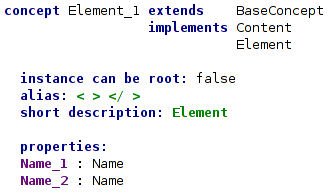
\includegraphics[scale=0.75]{./images/element_node_common.png}
	\caption{Resulting Element{\_}1 node}
	\label{fig:element_node_common}
\end{figure}

String literals (e.g., keywords such as \textbf{for}) are omitted/skipped because they will appear only in the corresponding projectional editor.
The node named \mpsconcept{Element{\_}1} contains two properties, one for each reference to the lexer rule \antlrlexerrule{Name} inside the first alternative of the \antlrparserrule{element} rule,
Value of the property will be restricted using the regular expression representing the \antlrlexerrule{Name} rule.
We explain later how the references to parser rules (\antlrparserrule{attribute} and \antlrparserrule{content}) as this is where the approaches differ.
The main/key difference between these two lies in the way we create children fields for parser rules and in the way we are going to link them together using interface concepts.

\subsubsection{The Straightforward Approach}
\label{sect:straightforward_approach}

The key idea of this approach is that, for each rule with more than one alternative, an interface node is created.
Consider the \antlrparserrule{content} rule from our SimpleXML language (Figure~\ref{fig:contentrule}).

\begin{figure*}[ht]
\centering
\begin{antlr}
	\antlrparserrule{content}    :   \antlrlexerrule{TEXT}
           |   \antlrparserrule{element}
           |   \antlrparserrule{comment}
           |   \antlrlexerrule{CDATA}
           ;
\end{antlr}
\caption{Content rule}
\label{fig:contentrule}
\end{figure*}

Any of the four nodes corresponding to alternatives could appear anywhere the \antlrparserrule{content} rule is referenced.
So we will create one interface node, and then for each alternative of this rule we create one node that implements the interface.
The resulting fragment of structure will look like the one in Figure~\ref{fig:icontentitf}.

\begin{figure*}[ht]
\centering
\begin{mps}
	\mpsinterface{IContent}   :   \mpsconcept{Content{\_}1}
           |   \mpsconcept{Content{\_}2}
           |   \mpsconcept{Content{\_}3}
           |   \mpsconcept{Content{\_}4}
\end{mps}
\caption{IContent interface}
\label{fig:icontentitf}
\end{figure*}

References to other parser rules are captured by links to children (interfaces or object nodes) in the AST nodes.
For the \antlrparserrule{element} rule that is referencing the \antlrparserrule{content} rule, defined as in Figure~\ref{fig:elementrule}, we get the AST node representing the first alternative that is shown in Figure~\ref{fig:element_node_full}.
There is one \mpsinterface{IElement} interface node that is implemented by two object nodes \mpsconcept{Element{\_}1}, \mpsconcept{Element{\_}2}.
The node \mpsconcept{Element{\_}1} has two child links pointing to \mpsinterface{IAttribute} and \mpsinterface{IContent}.

\begin{figure*}[ht]
\centering
\begin{antlr}
	\antlrparserrule{element}    :   \antlrliteral{<} \antlrlexerrule{Name} \antlrparserrule{attribute}* \antlrliteral{>} \antlrparserrule{content}* \antlrliteral{</} \antlrlexerrule{Name} \antlrliteral{>}
           |   \antlrliteral{<} \antlrlexerrule{Name} \antlrparserrule{attribute}* \antlrliteral{/>}
           ;
\end{antlr}
\caption{Element rule}
\label{fig:elementrule}
\end{figure*}

\begin{figure}[ht]
	\centering
	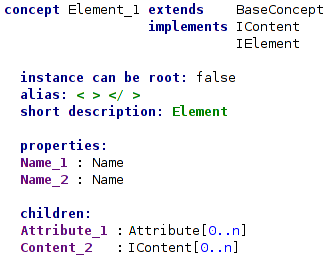
\includegraphics[scale=0.75]{./images/element_node_full.png}
	\caption{Element{\_}1 node's structure aspect}
	\label{fig:element_node_full}
\end{figure}

A problem with this approach, which we call \emph{the layer problem}, is related to the grammar rules (and corresponding AST nodes) that represent intermediary layers created only to make the grammar more readable.
The intermediary layers are created by authors of the grammars in order to make them more readable and more easily (better) maintainable.
We illustrate this problem (and explain it) on the behavior of auto-completion in MPS.
Imagine there is a freshly inserted \mpsconcept{Element{\_}1} node (representing the full XML element as is stated in the first alternative of the \antlrparserrule{element} parser rule).
Now we would like to insert another nested XML element inside.
MPS auto-completion mechanism would give us four options that are captured in the left part of Figure~\ref{fig:layer_problem}.
This is because there exist four nodes (objects) that implement the \mpsinterface{IContent} interface as per each alternative of the rule.

\begin{figure*}[ht]
	\centering
	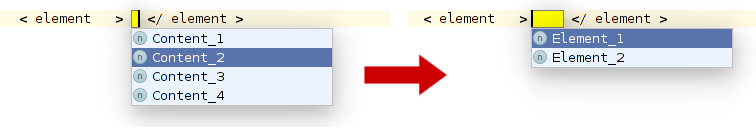
\includegraphics[scale=0.5]{./images/layer_problem.png}
	\caption{Layer problem in auto-completion}
	\label{fig:layer_problem}
\end{figure*}

However, in order to correctly insert another nested element inside, a user would have to first insert the \mpsconcept{Content{\_}2} node inside \mpsconcept{Element{\_}1} that has an \mpsinterface{IElement} child inside (and nothing else).
Then, as the second step, a user would invoke/trigger/call for the auto-complete again and insert either \mpsconcept{Element{\_}1} or \mpsconcept{Element{\_}2} inside \mpsconcept{Content{\_}2}.
This mean that a user would have to go through two steps, and in the first stepe either correctly guess (or remember the grammar rule's alternative order), which option/item offered by the auto-complete menu to select.

Similarly, if one would decide to replace the nested \mpsconcept{Element{\_}1} node with, let's say, an XML comment (a \mpsconcept{Comment} node), we need to delete both intermediary layers before we get back to the original \mpsconcept{Content{\_}X} selection (crossroads).
The user cannot really see what is happening, since the intermediary level has no appearance or indicator.
This may lead to confusion on the user's part.

The layer problem is solved/addressed by the second approach, which we describe in the next subsection.

\subsubsection{The Shortcut Approach}
\label{sect:shortcut_approach}

The key idea of this approach is to identify rules and nodes that are at the end of the (derivation, inheritance) chain, and offer them directly to the user through the auto-completion menu.
We call such \emph{end rules} and \emph{end nodes}, respectively, because they cannot transparently break into more rules/nodes.

\begin{figure*}[ht]
\centering
\begin{antlr}
	\antlrparserrule{content}    :   \antlrlexerrule{TEXT}
           |   \antlrparserrule{element}
           |   \antlrparserrule{comment}
           |   \antlrlexerrule{CDATA}
           ;

	\antlrparserrule{element}    :   \antlrliteral{<} \antlrlexerrule{Name} \antlrparserrule{attribute}* \antlrliteral{>} \antlrparserrule{content}* \antlrliteral{</} \antlrlexerrule{Name} \antlrliteral{>}
           |   \antlrliteral{<} \antlrlexerrule{Name} \antlrparserrule{attribute}* \antlrliteral{/>}
           ;

	\antlrparserrule{comment}    :   \antlrliteral{<!--} \antlrlexerrule{TEXT} \antlrliteral{-->} ;
\end{antlr}
\caption{Content parser rule with children}
\label{fig:contentrulewithchildren}
\end{figure*}

For example, the \antlrparserrule{content} rule, given in Figure~\ref{fig:contentrulewithchildren} together with its child rules, can ultimately expand into following nodes:

\begin{itemize}
	\itemsep0em
	\item \textbf{Content{\_}1} (TEXT)
	\item Content{\_}2 $\rightarrow$ \textbf{Element{\_}1}
	\item Content{\_}2 $\rightarrow$ \textbf{Element{\_}2}
	\item Content{\_}3 $\rightarrow$ \textbf{Comment}
	\item \textbf{Content{\_}4} (CDATA)
\end{itemize}

The end nodes are highlighted using the bold font.

Figure XY shows the algorithm (in pseudocode) that finds all end rules for a given parser rule.

% TODO pouzit standardni environment pro algoritmy 
\begin{figure*}[ht]
\centering
\begin{antlr}
	FindPathsToEndNodes($R$):
	1)  Define $L$ as an empty list of list of nodes
	2)  Return FindPathsToEndNodes($R$, $L$)

	FindPathsToEndNodes($R$, $L$):
	3)  Define $Q$ as list of list of nodes
	4)  For each alternative $A$ of rule $R$:
	5)      $L1$ = Clone($L$)
	6)      If $A$ is a parser rule with only one element $E$:
	7)          Let $I$ be interface/concept representing rule $E$
	8)          $L1$.Add($I$)
	9)          $P$ = FindPathsToEndNodes($E$, $L1$)
	10)         $Q$ = Merge($Q$, $P$)
	11)     Else
	12)         $L1$.Add($R$)
	13)         Let $P$ be concept representing $A$
	14)         $L1$.Add($P$)
	15)         $Q$.Add($L1$)
	16) Return $Q$
\end{antlr}
\caption{Algorithm for finding end rules}
\label{fig:shortcut_algorithm}
\end{figure*}

To find end rules for each parser rule, the algorithm recursively scans through the parser tree that was built before.
For each parser rule, it tries to find paths leading to some end rule through its alternatives:
\begin{itemize}
	\item Whenever it finds an alternative that contains only one element, and this element is a reference to another parser rule, it has found an intermediary level that can be transparently hidden from the user of the language.
		The process (algorithm) continues by recursively processing alternatives of this "level" rule (since we are not at the end of the chain yet).
	\item Otherwise, an end rule was found (recursion stops here).
\end{itemize}

By appending the rule that is leading to current element (line 12) and then appending that alternative's element itself (line 14), we get a path that contains the full path and the target end rule as the last element of the chain.
The result of this algorithm, for example for the \antlrparserrule{content} rule, equals the listing of the five paths mentioned above.

We do/repeat this for all parser rules and for each rule we get a list of paths that lead from that particular rule to an end node.
We call these paths as \textbf{shortcuts}, because they provide a shortcut from the rule to the end of the chain.
Now that we have the shortcuts, we will discuss several ways how to use the shortcuts (them) to improve the MPS language under construction (how to make the language better).

The primary use of shortcuts is to generate options for the auto-completion menus such that only the end nodes are offered.
This can be technically done in two ways --- (1) through custom auto-complete menus and deletion handlers or (2) by defining a special interface for each rule such that the interface is implemented only by end nodes for the rule.
Shortcuts have to be considered when inserting nodes but also when deleting them, i.e. the whole chain (shortcut path) consisting of possibly multiple intermediary AST nodes (levels) up to the end node must be added, respectively deleted.
The effect of insertion must be fully reversed when the user wants to delete some end node (the given end node).

\subsection{Editor}

When all types of AST nodes in the language are created, the next step is to define their visual representation in the projectional editor.
As stated before (in Section X (about JetBrains MPS, part of background)), MPS uses a cellular system that allows placing node's properties and children into a table-like arrangement.
Cells of different types are available --- for storing property values, references to child nodes, and keywords (string literals), and also cells that influence layout (e.g., indentation).

The purpose (goals) of this (third) step is to create the editor aspect for each language element.
It should project all attributes of the element --- name, properties, children, and so on --- using the respective cell types.

The main challenge (problem) here is that an input grammar (ANTLR) does not provide/give any help/aid/information regarding the code layout.
As we already said in the introduction, one of the biggest challenges/problems that arise here is that the grammar description of a language does not hold any information about the code layout.
The structural rules in the grammar only tell us, what the syntax tree looks like and how the code is broken into nodes.
In particular, the grammar says nothing about indentation, line breaks, and another formatting.

We tackled this problem by designing an automated learning approach, which generates the layout using several heuristics.
We present our solution to this problem. It involves some intermediary step whose purpose is to generate the necessary information.
Our solution is semi-automated (using some heuristics) --- user's help in an interactive manner is needed for final touches (polishing).
It works as follows.

As input for the algorithm (learning approach), the user has to supply to a set of valid source files written in the imported language, together with the grammar file.
These four steps/operations are then performed.
\begin{enumerate}
	\item Automated generation of an ANTLR parser for the input language using the ANTLR library.
	\item Modify/extend the code of the generated parser in order to record some additional information.
	\item Compile the parser into an executable form.
	\item Use the parser to parse the supplied source code files and extract information about the layout of the code during this process.
\end{enumerate}
This way, the imported/created MPS language would inherit the code style/layout directly from the user, i.e. it would learn directly from the code.
In step 2, the parser is modified such that it remembers/stores the line number and column for each parsed token.
This is very efficient and it enables to create a nice layout.
From the line number, the algorithm can easily determine whether there is a line break between some tokens (statements, language elements).
The column number can be then used to detect indentation.
However, this approach is still heuristic and may give imprecise (suboptimal) results --- mainly because it is not always possible to precisely match language elements (in the MPS structure) with all tokens that belong to it.
Note also that quality of the extracted information always depends on the amount of the source code files provided (available, supplied) and on how representative the set of source code files actually is.
When our algorithm cannot determine some custom layout, it just creates all the cells (content) of the editor aspect and arranges them in a single row.
Figure~\ref{fig:editor_adjustment} XY shows the difference between the default single-row layout (in the upper left corner) and the fully customized layout (in the bottom right corner) for the \mpsconcept{Element{\_}1} node.

% TODO smazat cervenou sipku z toho obrazku a mozna rozdelit na dve casti (vlozit tam caru): default single-row code layout, optimal fully customized layout
\begin{figure*}[ht]
	\centering
	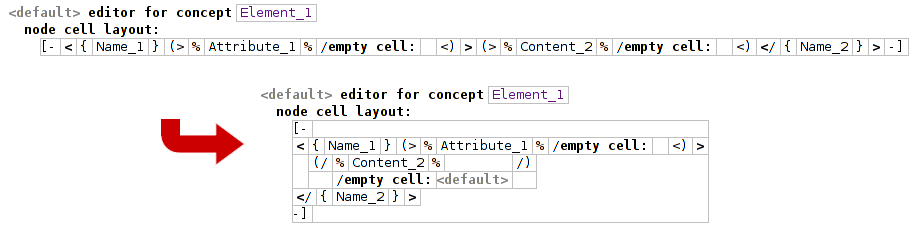
\includegraphics[scale=0.5]{./images/editor_adjustment.png}
	\caption{Projectional editor adjustment of the Element{\_}1 node}
	\label{fig:editor_adjustment}
\end{figure*}

In practice, however, the user still has to tweak the editor aspect --- to adjust the code layout --- because the heuristics are not 100\% reliable.
But it takes a very short time to reach optimal results (because MPS allows doing this very efficiently), as we show on the example of importing the JavaScript language~\cite{ref:javascript} and manually adjusting all editors that needed it, all that in a less than hour time.
More details are provided later in Section X (examples) --- there we describe this issue further.

\subsection{Text Generation}

The final/last, fourth step, is to create the TextGen aspect for each AST node.
The purpose of the TextGen aspect is to define, for a language element (AST node), what code in the BaseLanguage will be generated out of it, once we want to compile and run our MPS code/program.
This is needed to allow/enable users to generate plain-text source code representation out of the AST they built/created inside MPS.
Again, a TextGen aspect must be created for each language element.
Basically, it is a single method in the BaseLanguage (or in Java?) for each language element.
The method generates a string (plain-text) representation of the element, appends the string to the output stream, and then calls TextGen methods on all children of the element.

A very basic example of BaseLanguage code that can be used as the TextGen aspect of an \mpsconcept{Element{\_}1} node, which represents the full XML tag with content, is shown in Figure~\ref{fig:textgen_example}.
It appends all literals, properties, and children in the same order as they appear in the grammar definition.

\begin{figure}[ht]
	\centering
	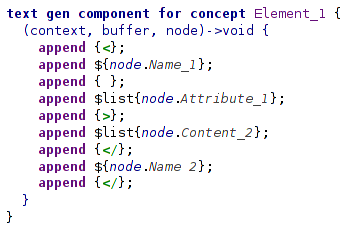
\includegraphics[width=90mm]{./images/textgen_example.png}
	\caption{Example of a~TextGen aspect}
	\label{fig:textgen_example}
\end{figure}

Like in the case of editor, we discovered some interesting challenges related to the code layout, whitespaces, and more (so on).
We describe our solution to the challenges here in this section.

The reader might have noticed that there is no whitespace handling inside of our SimpleXML grammar (Section XY, running example).
Grammars in the ANTLRv4 notation are usually written in such a manner that whitespace characters are skipped (ignored).
However/Nevertheless, TextGen aspect (generator) should/must know between which children there must be a whitespace and where it is forbidden (i.e., where to put some whitespace characters) so that the produced code is a valid one.
For example, in the case of the \antlrparserrule{element} rule, TextGen must determine that there should be a space in between \antlrparserrule{attribute} and \antlrlexerrule{Name}, while it is not required between \antlrliteral{\textless} and \antlrlexerrule{Name}.
In general, it is sufficient to put just a single space character at places/locations where there has to be some whitespace in order to make the code valid (syntactically correct).

Layout of the generated code is also important. For example, the user may want to produce more readable code by adding indentation or line breaks.

In fact, the problem of TextGen layout is quite similar to the one we have seen with the projectional editor, described in Section XY.
Since we are dealing mostly with text-based languages, their representation in projectional editor must be almost the same as their expected plain-text representation (output).
Therefore, one could use the same approach for editor and TextGen --- adding line breaks and indentation.
Once we would have some information about the layout for generating better projectional editor, we could leverage the same information and use it to improve TextGen.

Nevertheless, in our current approach, the editor aspects have to be adjusted manually, after the import is done, because for now it is the fastest and the most efficient way how to deal with the problem of customizing the editor to capture a nice layout.
Therefore, we used a different approach for TextGen --- a really simple heuristics which gives surprisingly good results.
In the first step, a very basic TextGen is created that inserts spaces in between every two tokens of the language element (AST node).
Then, as the second step, spaces are eliminated (restricted) from positions where they are not really needed.
We describe all the cases here:

\begin{enumerate}
	\item Whenever there is a non-alphabetical literal,	appearing as a plain string token defined in the grammar, that might get recognized by the parser safely without the need for a whitespace separator around, then we omit spaces around it.
		For example, consider \textbf{'\textless'} in SimpleXML.
	\item Another group are strings inserted by the user of the language, whose form is constrained by a regular expression.
		For example, an XML tag's name belongs to this group.
		They are usually values of properties defined in structure aspects.
		A space must be preserved only when a neighboring literal may end with an alphabetical character. Otherwise, we can omit the space.
		In practice, this will eliminate redundant spaces inside of quotes, next to semicolons, and around brackets, but, on the other hand, it will separate language keywords (function, var, in, etc.) from other content by keeping the space character in between them.
	\item Spaces are omitted also in the case of child nodes that are not present (e.g., when they are optional), and in the case of empty lists of child nodes, so that spaces do not accumulate.
	\item On the other hand, when two child elements are next to each other, we always insert space.
	\item Sequences of children are separated with space or with a line break.
\end{enumerate}
These few simple heuristics work surprisingly well and give us some very nice results.
We discuss our experience with XML, JSON, and JavaScript in Section XY (Evaluation).

Figure~\ref{fig:textgen_final} shows an example of a TextGen aspect for the full SimpleXML element.

\begin{figure}[ht]
	\centering
	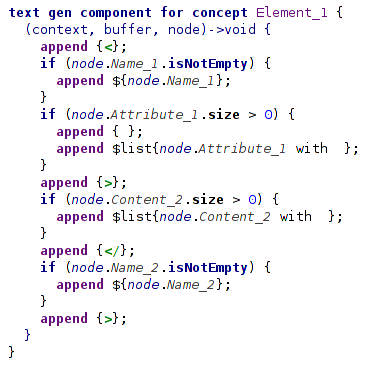
\includegraphics[width=95mm]{./images/textgen_final.png}
	\caption{Generated TextGen aspect for the SimpleXML element}
	\label{fig:textgen_final}
\end{figure}

The automatically generated TextGen code can be adjusted manually very easily, so that it generates nicely indented XML code.
In the case of the example above (in Figure F), we only need to wrap the \mpsconcept{Content{\_}2} child with indentation and change the sequence separator to a new line character.
The resulting adjusted aspect (code) is shown below in Figure~\ref{fig:textgen_adjusted}.

\begin{figure}[t!]
	\centering
	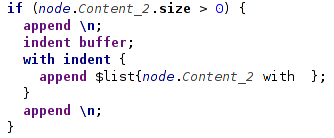
\includegraphics[width=85mm]{./images/textgen_adjusted.png}
	\caption{Adjusted indentation inside the TextGen aspect}
	\label{fig:textgen_adjusted}
\end{figure}

\subsection{Remarks about Grammars}

As we have already shown in previous sections, it is very easy to write a grammar in a way that will cause problems during import into MPS (or once it is imported).
Problems might occur during the creation of any aspect.
Here we will look at some general problems/issues that grammar import poses (might pose).
We will talk about these problems with respect to the challenges/obstacles we tried to overcome and which we described in previous sections (dedicated to structure, editor, and texgen, respectively).
We also show a few examples of additional possible complications.

\paragraph{Adjusting grammars.}
There are some cases, where altering the input grammar might yield far better MPS language.
We will show two examples how the usability of the resulting MPS language can be improved.
Let us look at the definition of an XML attribute in Figure~\ref{fig:xmlattribute}.

\begin{figure*}[ht]
\centering
\begin{antlr}
	\antlrparserrule{attribute}   :   \antlrlexerrule{Name} \antlrliteral{=} \antlrlexerrule{STRING} ;
	\antlrlexerrule{STRING}      :   \antlrliteral{"} \antlrregex{~["]*} \antlrliteral{"}
	            |   \antlrliteral{\textbackslash'} \antlrregex{~[']*} \antlrliteral{\textbackslash'}
	            ;
\end{antlr}
\caption{Definition of an XML attribute}
\label{fig:xmlattribute}
\end{figure*}

The original XML grammar has quotes as a part of the value.
For the resulting MPS language, it would mean that there would be a placeholder for the attribute value that would expect us to input the leading and trailing quote together with the value too each time.
It would also be marked red (by the syntax checker) unless we enter both quotes inside the value since the regular expression checking for quotes will not match.
The user might be confused by this and will not be able to tell why his string value is incorrect.

In our SimpleXML language, we adjusted the grammar easily in the manner that we show in Figure~\ref{fig:xmladjustgrammar}.

\begin{figure*}[ht]
\centering
\begin{antlr}
	\antlrparserrule{attribute}   :   \antlrlexerrule{Name} \antlrliteral{="} \antlrlexerrule{TEXT1} \antlrliteral{"}
	            |   \antlrlexerrule{Name} \antlrliteral{=\textbackslash'} \antlrlexerrule{TEXT2} \antlrliteral{\textbackslash'}
	            ;
	\antlrlexerrule{TEXT1}       :   \antlrregex{~["]*} ;
	\antlrlexerrule{TEXT2}       :   \antlrregex{~[']*} ;
\end{antlr}
\caption{Adjusted grammar of SimpleXML}
\label{fig:xmladjustgrammar}
\end{figure*}

We turned quotes into literals, thus ensuring that they will only appear in the projectional editor as fixed constant cells.
We will not have to encapsulate the value in them each time.
The user will only have to choose, which attribute version he wants to use (single or double quotes).

As the second example, we will show the ECMAScript\footnote{https://github.com/antlr/grammars-v4/blob/master/ecmascript/ECMAScript.g4} language otherwise known as JavaScript.
Every statement in JavaScript needs to be either followed by a semicolon, newline, file end or end of the block --- see the Figure~\ref{fig:javascriptstmt}.

\begin{figure*}[ht]
\centering
\begin{antlr}
	\antlrparserrule{eos}            : \antlrlexerrule{SemiColon}
	               | \antlrlexerrule{EOF}
	               | {lineTerminatorAhead()}?
	               | {{\_}input.LT(1).getType() == \antlrlexerrule{CloseBrace}}?
	               ;
	\textcolor{gray}{// Example reference of the eos rule}
	\antlrparserrule{breakStatement} : \antlrlexerrule{Break} \antlrlexerrule{Identifier}? \antlrparserrule{eos}
	               ;
\end{antlr}
\caption{Statements in JavaScript}
\label{fig:javascriptstmt}
\end{figure*}

Because there are multiple options, our import plugin would create a placeholder at the end of every statement.
Every language element representing a statement would have one child of the \mpsinterface{IEos} interface type.
This placeholder needs to be manually filled in for each statement.

Since the projectional editor has much bigger power over the form of the code, we (a user) might want to have each statement on a separate line.
Since we can differentiate between statements on the AST level, we do not need an explicit separator between them.
This means that we might want to simplify the language and leave the semicolon out, or leave it just as a constant fixed part of the projectional editor, but not as something the user must explicitly fill in.
Then we can just put each statement on a separate line as it is usual for JavaScript code, but we do not need the semicolon anymore.
This small adjustment is very quick when done inside the grammar.
We just change the \antlrparserrule{eos} rule to the form shown in Figure~\ref{fig:eosrule}.

\begin{figure*}[ht]
\centering
\begin{antlr}
	\antlrparserrule{eos} : \antlrliteral{;} ;
\end{antlr}
\caption{eos parser rule}
\label{fig:eosrule}
\end{figure*}

This way, we can change the grammar in a way that it will not describe the same ECMAScript language as before, but will definitely make our MPS language more usable.
TextGen aspect may be defined in such a way that puts the semicolon back (after each statement) in the generated plain-text representation. 
This would be very important especially when JavaScript is available as another base language (which is actually a plan (future work) of the JetBrains company).

Above, we have shown that adjusting the input grammar might be a very fast mean of tweaking/improving the usability of generated MPS language, and sometimes it may be the only proper solution in some complex situations.
In general, the question we can ask ourselves is whether one aims for a full precise/faithful port of the input language or for an MPS alternative.

\todo{Nahradit slovo "break" v nasledujicich odstavcich (v kontextu "break the parser") za vhodnejsi slovo ktere pusobi vic odborne.}

\paragraph{Breaking grammars and parsers.}
However, we have found that there is one big problem with grammar adjustment that we would like to point out.
The problem is that it is very easy to change the input ANTLR grammar in a way that breaks the ANTLR parser generated out of it.
By breaking we mean that it stops parsing the original language.
We illustrate the problem on our SimpleXML language.

As stated before, when creating the SimpleXML grammar, we have started off with the original XML grammar\footnote{https://github.com/antlr/grammars-v4/tree/master/xml} and did some adjustments to it.
We ended up with a grammar that can be processed by our method/plugin and creates a nice usable MPS language.
Nevertheless, we noticed that even though the imported language behaves well enough and mimics the XML language quite nicely, the ANTLR parser generated out of this grammar no longer parses XML successfully.
Some changes we have made, such as the attribute adjustment, broke the grammar down.
More precisely, our changes improved the MPS language while breaking down the parser, and we have not even noticed it because, from the perspective of MPS, the imported language still corresponds to XML.

What we are trying to say (show here) is that it is very easy to perform a grammar adjustment that will, at first, seem harmless and valid inside MPS, but will break the parser.
The problem is that the user performing this change probably will not be aware of breaking it.

The main (underlying) cause of this problem is the way the ANTLR parser is implemented and the quite different purpose we are using the grammar for in our project/tool/method.
There are many ways how various parsers deal with, for example, token matching.
For instance, ANTLR introduces so called \emph{greedy} and \emph{non-greedy} operators.
The greedy way, in which ANTLR matches input on defined tokens and prioritizes their selection, makes some rules very dangerous.
When a rule matches a wide range of input, it might happen during parsing that it is prioritized over other rules and swallows a lot more input than the author of it intended.
Usually, these dangerous rules are bound to some parser context, which makes them behave well.

However, for practical reasons, it is very important that grammar is not broken by our custom adjustments (and that the ANTLR parser of the language works properly), because we might need to automatically generate parsers of the adjusted language.
Imagine this very real scenario (that will be supported in the future):
\begin{enumerate}
	\item We have imported the language inside MPS.
	\item MPS now knows the structure of the language, and we can code in MPS using this language.
	\item We would expect MPS to be able to load an existing source code, written in this language, from a text file and import it inside MPS.
	\item We would like to use MPS to safely edit this code, using all the features of MPS.
	\item We would also like to export the code in a plain-text form again and save it back to the source file.
\end{enumerate}
In order to make this happen, we must be able to generate a correctly-working ANTLR parser out of the adjusted source grammar that we used to (that helped us) import the language.
We must also be able to match nodes of the AST coming out of the ANTLR parser to elements of the MPS language, and we must build the MPS AST out of the ANTLR AST.


\section{Evaluation}

We implemented everything (the proposed approach described above) in the form of an MPS plugin that allows users to carry out the import.

We used a mix of Java and BaseLanguage in our implementation.
We used the MPS API, which can be called from the BaseLanguage programs too, to generate some of the language elements.
BaseLanguage is needed to use/call the MPS (language) API, i.e. to programmatically create new language elements and their aspects.

The plugin uses the ANTLR library to work with ANTLRv4 grammar files (to parse them, etc) and several MPS libraries (that implement the MPS API).

For the first step of automated construction of MPS languages from grammars (i.e., for parsing the grammar), the plugin uses the ANTLR library~\cite{ref:ANTLR4} to generate a Java ANTLR parser of the ANTLRv4 notation, because there exists an ANTLRv4 grammar for the ANTLRv4 notation~\cite{ref:ANTLR4reference}.

\todo{
	We should provide url to the github repository (implementation) and pointer to some package with ANTLR grammars and imported MPS languages (take from Attachments.zip in the master thesis).
}

\todo{Popsat nase zkusenosti s importem slozitych jazyku (XML, JavaScript, Python, a dalsi).}

From introduction: We will also show some example languages imported with INGRID and discuss our experience.

In order to evaluate INGRID, we tried to import several real/mainstream languages:
\begin{itemize}
	\item \textbf{SimpleXML} --- Simplified XML that we used in this thesis for explanatory purposes.
	\item \textbf{JSON} --- Similar to XML, but this time a full port of the specification.
	\item \textbf{ECMAScript 5.1} --- Specification of the language known as JavaScript, dated to the year 2011, which is currently the most frequently adopted version.
\end{itemize}
Results of the import process are included in the package that is available at \todo{url}.
The repository \todo{Add url} contains an example MPS project. There are three languages.
For each example language, you can find its original import, exactly in the form as created by our plugin.

We experimented with import of XML, JavaScript, Python, and maybe some other languages.

These general purpose languages are quite complex when it comes to their structure and the overall syntax variety.

We must emphasize that the automatically imported languages are not ready-to-use full-fledged MPS languages.
We did not expect to achieve that at this stage, as that is a much bigger, if not impossible, challenge.
Imported languages contain full structure found in the respective grammars and some more aspect definitions that will help users of the languages in creating code.
The imported language has to be manually adjusted (tweak, polished) by the end user (developer) and some of its complications have to be resolved manually by a human.

We found out that manual adjusting of the editor/textgen aspect (adding line breaks and indentation) is far more effective and precise than any automated approach we came up with (during our research).
The imported language can be, in our opinion, adjusted very fast into a more readable form.

The package at \todo{url} contains also adjusted versions of all three languages.
Then, for each language, there is an adjusted version.

This adjusted version was created from the original import and the author spent no more than between 20 to 60 minutes of working on it.
The first author spent only a couple of minutes of (manually) adjusting them after the automated import, so that we try to prove our point above.
More specifically, the JSON language was ready for use in no more than 20 minutes of minor adjusting.
We chose this language because it does not require us to implement complex aspects, such as type checking or data flows.
Similarly, the SimpleXML turned out very nice.

Our main goal was to prove that even though our method (plugin) does not create a perfect language, it can be customized very fast into a very usable form.
We manually tweaked/customized the editor and the TextGen aspect only, structure aspect was left in its original form.
This justifies some of the decisions we have described in Section X (editor aspect) and Section Y (textgen), proving that our approach is quite practical (and the best).

We have also tried to use the INGRID tool/plugin to import the JavaScript language, which is exactly the type of a complicated general purpose language that might be of interest to other people.
There are already some projects, where a manual port of JavaScript is being done.
One of them is the ECMAScript4MPS~\cite{ref:ECMAScript4MPS} from the author of the PE4MPS project~\cite{ref:PE4MPS} that we described in Section X (similar projects, related work).
The result of import by INGRID is quite good, comparable to the PE4MPS project.
Our language is, of course, missing a lot of more advanced aspects/features that, for example, can help deriving types of expressions and so on.
These aspects improve the usability by a lot, e.g. when the user starts writing numbers, a number literal is inserted, whereas in our import the user has to first insert the concept representing the number literal and then proceed with writing numbers.
These actions are needed in any MPS language and are expected to be implemented after the import step, \todo{Maybe say that INGRID does not generate these actions/aspects/features yet but it is our future work} as it is not possible to generate them automatically.
However, when it comes to language structure, concept aliases, and auto-completion, we think that INGRID (our method/plugin) did a very good job.
The structure aspect is very similar to the ECMAScript4MPS's one, which was created manually over the course of a large number of hours.
INGRID does that (achieves the same result) fully automatically.

To summarize, import languages such as JavaScript, JSON, MySQL and others is giving nice results.

Results of our experiments with languages such as JSON or JavaScript show that the proposed approach (INGRID) yields very good results, comparable to existing manual ports, and spares the user from hours of tedious, error prone and time-consuming work.

Limitation: the project is lacking proper error reporting and cannot handle cyclic rules (which could be found in Python grammar, for example).


\section{Conclusion and Future Work}

\todo{Write something.}

There is lot of further follow-up work to be done. Many open problems remain.

Automated generation of the editor aspect, probably using some kind of machine learning.
Generating nicely designed and user-friendly editors, maybe using artificial intelligence (machine learning) that would evaluate (analyze) existing code in plain text and based on that create the editors.

Follow-up work might look more into the problem of code layout detection, possibly exploring suggested approaches such as the learning approach described in Section XY \todo{Tohle se snad podari aspon castecne implementovat}.
This could lead to better results in editor and TextGen aspect generation which could definitely use some improvement.
Another future endeavors will definitely touch the subject of generating parsers that would enable the user to import existing source code into MPS.



\acks
% TODO
This research was supported by JetBrains. \todo{Pridat jeste nejaky grant a kompletne preformulovat.}

\bibliographystyle{abbrvnat}

% TODO opravit formatovani jednotlivych zaznamu a vhodne seradit
\begin{thebibliography}{}

\bibitem{ref:MPS} JetBrains MPS, \url{https://www.jetbrains.com/mps/}

\bibitem{ref:mbeddr} mbeddr, \url{mbeddr.com/}

\bibitem{ref:BaseLanguage} BaseLanguage, \url{confluence.jetbrains.com/display/MPSD34/Base+Language}

\bibitem{ref:PE4MPS} PE4MPS project, \url{https://github.com/mar9000/pe4mps}

\bibitem{ref:PE} PE project, \url{https://github.com/mar9000/pe}

\bibitem{ref:ANTLR2MPS} ANTRL{\_}MPS project, \url{https://github.com/CampagneLaboratory/ANTLR{\_}MPS}

\bibitem{ref:ANTLR4} ANTLRv4, \url{https://github.com/antlr/antlr4}

\bibitem{ref:ANTLR4reference} T. Parr. The Definitive ANTLR 4 Reference. The Pragmatic Bookshelf, 2013

\bibitem{ref:ANTLR4grammars} ANTLRv4 grammar repository, \url{https://github.com/antlr/grammars-v4}

\bibitem{ref:ECMAScript4MPS} ECMAScript4MPS project, \url{https://github.com/mar9000/ecmascript4mps}

\bibitem{ref:javascript} JavaScript ANTLRv4 grammar, \url{https://github.com/antlr/grammars-v4/blob/master/ecmascript/ECMAScript.g4}

\end{thebibliography}

\end{document}

